\documentclass[paper=a4,11pt,bibliography=totoc]{scrartcl}
%\usepackage{fourier}

\usepackage[utf8]{inputenc}
\usepackage[english]{babel} 
%\usepackage[round,sort,authoryear]{natbib}
\usepackage{hyperref}
\usepackage{url}
\usepackage[protrusion=true,expansion=true]{microtype}
\usepackage{amsmath,amsfonts,amsthm}
\usepackage[pdftex]{graphicx}
\usepackage{subfigure}
\usepackage{longtable}
\usepackage{float}
\restylefloat{table}
\usepackage{tabularx}
%\usepackage{todonotes}
\usepackage{booktabs}
\usepackage{framed}
\usepackage{listings}
%\usepackage{newclude}
\usepackage{enumerate}
\usepackage{color}
\usepackage{setspace}
%\onehalfspacing
\parskip 3mm
% Verhindert die Einrückung der Absätze
\setlength{\parindent}{0pt}

\usepackage{xcolor}
\hypersetup{
    colorlinks,
    linkcolor={red!50!black},
    citecolor={gray!80!black},
    urlcolor={gray!80!black}
}

\newcommand*{\fullref}[1]{\hyperref[{#1}]{\ref{#1} \nameref*{#1}}}

\setcounter{secnumdepth}{5}
\setcounter{tocdepth}{5}

\title{\vspace*{5cm}\onehalfspacing{Visualization, Reconstruction and Processing of Point Clouds}}
\subtitle{\vspace*{1.4cm}\onehalfspacing{Possibilities and constraints of the\\Point Cloud Library (PCL) and the Three.js library}\\[0.5in]University of Heidelberg\\-- Project report --\\Softwarepraktikum (2015/2016)}

\author{Lukas Kades}

\date{\today}

\begin{document}
\maketitle
\thispagestyle{empty}
\newpage
\setcounter{page}{1}
\renewcommand{\contentsname}{I Contents}
\renewcommand{\refname}{II References}
\addcontentsline{toc}{section}{I Contents}
\tableofcontents

\newpage 

\definecolor{darkgreen}{rgb}{0,0.39,0} 
\definecolor{darkred}{rgb}{0.39,0,0}
\definecolor{lightblue}{rgb}{0.063,0.14,0.59}

\section{Project description}
\label{sec:projectdescription}
%
In these days recording a depth image with a kinect camera is not unusual anymore. It arises however the question, which programs are most suitable for illustrating the depth data together with the color image in an appropriate 3D surrounding. Furthermore it is an enormous task to generate a connected mesh out of the point cloud. Of course certain programs like MeshLab are available, but despite these programs there are certain open project libraries which provide a vast amount of possibilities, not only for surface reconstruction and meshing, but also for other tasks in the wide range of image processing.

In this project possibilities and constraints of two open projects are explored, the Point Cloud Library (PCL) and the Three.js library. The main focus is based on the illustration of point clouds and the surface reconstruction and normal estimation methods respectively. PCL is written in C++ and offers a host of different possibilities for image processing. In contrast Three.js is mainly suitable for illustrating 3D data in a fast easily usable way with javascript in an html framework. The powerful javascript library provides furthermore many useful tools concerning reality effects like reflection, shadow, fog, etc., different textures and geometric basic objects, which makes it attractive for certain applications in webdesign and advertising.

After a short introduction of the different subtasks and obstacles during the working process of the project, it follows a detailed description of the different steps, methods and programs for the process of reading the raw data to an adequate application for illustrating the resulting rendered mesh. Problems, advantages, potential expansions and suggestions for improvement are given in the last section.
%
\section{Project structure and workflow}
\label{sec:projectstructure}
%
To get an insight into the workflow during the project this sections reveals the different stages and subtasks which have been run through during the project.

\textbf{Stage 1: Data praparation for PCL}
\begin{center}
\leftskip4em\small We used the NYU Depth V2 database which can be downloaded from \url{http://cs.nyu.edu/~silberman/datasets/}. The RGBD data was preprocessed with the help of Matlab and saved as undistorted images with depth information as well as color information.
\end{center}
%
\textbf{Stage 2: Visualization of point clouds in PCL}
\begin{center}
\leftskip4em\small After having successfully installed the necessary libraries in C++ and getting the first test program running (following the instructions of~\cite{peris}), the main task consisted in a correct illustration of the colored point cloud.
\end{center}
%
\textbf{Stage 3: Methods for processing RGBD data in PCL}
\begin{center}
\leftskip4em\small At this working step several tools for cropping, illustrating and creating the point cloud were written. Furthermore methods from PCL for estimating normals and reconstruct the surface were implemented. The resulting mesh, normals and cloud can be saved as ply-files in an appropriate format for further processing with other tools.
\end{center}
%
\textbf{Stage 4: Getting used to Javascript and Three.js}
\begin{center}
\leftskip4em\small For being able to work with Three.js at least an basis knowledge of html and javascript programming is necessary, which was gained by reading some example codes of Three.js and other simple tutorials as well as trying own little applications.
\end{center}
%
\textbf{Stage 5: Illustrating 3D data as html application using Three.js}
\begin{center}
\leftskip4em\small Following the style and concept of an already implemented depth data viewer~\cite{depthplayer} a similar user interface was developed, which covers the possibilities of loading and illustrating the 3D data, meshing the point cloud as additional method out of a plane over the image and smoothing the cloud by blurring the depth image.
\end{center}
%
A more detailed description of the different stages is given in the next sections with an emphasis on theoretical aspects concerning the different methods and on an explanation of how to work with the different functions.
%
\section{Preparation of the dataset}
%
As dataset NYU Depth V2 dataset from \url{http://cs.nyu.edu/~silberman/datasets/} is used. For handling the data a toolbox written in Matlab is provided from Silberman. In this section the file structure is explained as well as the necessary steps for praparation of the raw data for an usage with PCL. 
%
\subsection{File Structure}
The folder \textit{project} contains all necessary files, except the PCL and OpenCV libraries, which has to be installed separately. The documentation can be found in \textit{doc}, the \textit{CMakeLists.txt} file in the folder \textit{cmake} and the executables for PCL in \textit{bin}. The folders \textit{include} and \textit{src} contain all necessary header and C++ files for processing with PCL. In the folder \textit{lib} the javascript libraries are stored. The main file for visualization with a web browser is \textit{depthdataviewer.html}. Since handling data with javascript is not so easy and there are many different data files generated due to different operations, all data is stored in the folder \textit{data}.
%
\subsection{Generate depth and color images with Matlab}
\subsubsection*{\color{darkgreen}Theorectial issues}
%
With the help of the Matlab toolbox the through the camera distorted depth and color images, initially stored as raw data in \textit{data/rawdata}, are translated via Matlab into undistorted images and saved in the file formats: \textit{filename\_depth.pgm} and \textit{filename\_rgb.ppm} at \textit{data/undistfiles}.
%
\subsubsection*{\color{darkred}Implementation and usage}
%
\begin{itemize}
\item \textbf{\texttt{function [depthOut, rgbUndistorted] = project\_depth\_map(imgDepth,\\rgb)}}
\end{itemize}
%
\subsection{Interpolate depth data}
\subsubsection*{\color{darkgreen}Theorectial issues}
%
A problem that should not be underestimated is the occurance of pixels with missing depth data of the depth image. Since for many processing operations an organized point cloud is necessary or at least helpful, one has to find a way to handle with these points. Unless otherwise noted, it is worked with organized pointclouds in this project.
%
\begin{center}
\begin{minipage}[t]{0.8\textwidth}
\small\color{lightblue}\textsf{'An organized point cloud dataset is the name given to point clouds that resemble an organized image (or matrix) like structure, where the data is split into rows and columns. Examples of such point clouds include data coming from stereo cameras or Time Of Flight cameras. The advantages of a organized dataset is that by knowing the relationship between adjacent points (e.g. pixels), nearest neighbour operations are much more efficient, thus speeding up the computation and lowering the costs of certain algorithms in PCL~\cite{ordered}'.}
\end{minipage}
\end{center}
%
One possiblity is to set these points with missing depth data to $(0, 0, 0)$, accordingly they do not occur in the point cloud and are placed at the camera position. However, for processing with, for example, nearest neighbours on the basis of an organized point cloud, these shifted points distort the point cloud manifestly due to wrong resulting spatial distances, which makes an error-free application of normal estimation and mesh reconstruction very difficult.

A solution to this problem is to interpolate the depth image data in advance. For simplicity an algorithm was chosen which takes only the upper, left, lower and right neighbour into account. The updates are executed parallel and independent according to the arising number of neighbours with depth information, where points with a higher number of neighbours with depth data are updated first.
%
\subsubsection*{\color{darkred}Implementation and usage}
%
\begin{itemize}
\item \textbf{\texttt{void interpolateDepthData(std::string filename, std::string\\newfilename)}}\\
\textsf{The depth image \textit{filename} is loaded, the pixels with missing depth data are interpolated and the adjusted depth image is written to a file with \textit{newfilename}}.
\end{itemize}
%
\section{Point Cloud Library - Main written programs and functions}
%
The PCL point cloud library is as a highly-developped library for image and point cloud processing. The framework maintains numerous state-of-the-art algorithms including filtering, feature estimation, surface reconstruction, registration, model fitting and segmentation~\cite{pcldoc}. Some of these algorithms are used and tested for surface reconstruction and filtering of the depth data.
%
\subsection{Main program}
%
The main file \textit{main.cpp} includes all necessary headers and contains the main program for point cloud processing using the PCL library. Its executable is placed in the folder \textit{bin}. A small terminal based menu is written for an straight forward application of the implemented methods. The main menu is implemented in the class \textit{cloud.cpp} and included via \textit{cloud.hpp}.
%
\subsection{Creation}
\subsubsection*{\color{darkgreen}Theorectial issues}
%
The necessary functions for creating a point cloud out of the depth and color images can be found in \textit{creation.cpp} and are included via \textit{creation.hpp}. For a correct reconstruction of the 3D scene some intrinsic camera parameters (focal length, principal point) are needed. These parameters ar provided by the dataset and are stored in an extra file \textit{cameraparameters.txt} in the folder \textit{data}. For another dataset they have to be adjusted.

The reconstruction of the 3D scene out of the two-dimensional depth and color data is executed with the help of the focal lengths $fx\_d$, $fy\_d$ and the principal point $cx\_d$, $cy\_d$. Through the prepcrossing the depth coordinate (z-coordinate) can be loaded directly from the depth image and the spatial extension in x and y direction is computed via the pinhole camera model with:
%
\begin{equation}
\begin{pmatrix}
u\\v
\end{pmatrix}
\;=\;
\begin{pmatrix}
f_x/z & 0 & c_x \\
0 & f_y/z & c_y
\end{pmatrix}
\begin{pmatrix}
x\\y\\1
\end{pmatrix}\,,
\end{equation}
%
where x, y, and z are the depth values in meter and u and v correspond to the image indices.
%
\subsubsection*{\color{darkred}Implementation and usage}
%
\begin{itemize}
\item \textbf{\texttt{void createPointCloud (pcl::PointCloud<pcl::PointXYZ>::Ptr \&pcptr,\\std::string filename, int scale)}}\\
\textsf{The depth image \textit{filename\_depth.pgm} is loaded and with help of the focal lengths $fx\_d$, $fy\_d$ and the principal point $cx\_d$, $cy\_d$ a point cloud without color information (white) is contructed with a correct scale in all directions ($d$ stands for 'depth'). The pointer \textit{pcptr} points to the point cloud. The additional parameter \textit{scale} is introduced, which can be used to downsample the point cloud for a better perfomance for later processing operations. At the moment the width and the height of the two dimensional image have to be multiples of the width and height of the organized point cloud. This should be adapted to arbitrary scales.}
 
\item \textbf{\texttt{void createPointCloud (pcl::PointCloud<pcl::PointXYZRGB>::Ptr\\\&pcrgbptr, std::string filename, int scale)}}\\
\textsf{In addition to the previous function the color image \textit{filename\_rgb.ppm} is loaded as well and the organized point cloud structure makes it possible to easily assign the rgb-colors to the points. The pointer \textit{pcrgbptr} points to the point cloud.}
 
\item \textbf{\texttt{pcl::PointCloud<pcl::PointXYZRGB>::Ptr colorPointCloud\\(pcl::PointCloud<pcl::PointXYZ>::Ptr \&pcptr, std::string filename)}}\\
\textsf{Returns a pointer  to the colored point cloud. The colored point cloud is generated like in the previous function out of the uncolored point cloud.}
 
\item \textbf{\texttt{pcl::TextureMesh textureMesh(pcl::PolygonMesh \&mesh, std::string\\ filename, int scale)}}\\
\textsf{Projects the rgb-image on the constructed input polygon mesh and returns the textured mesh. Only applicable, if an rgb-image is available.}
\end{itemize}
%
\subsection{Visualization}
\subsubsection*{\color{darkgreen}Theorectial issues}
%
The PCL library provides a class for visualizing the created point clouds. Since for different 3D objects different functions are used, the functions for illustration are summerized in \textit{visualization.cpp} and are included via \textit{visualization.hpp}.
%
\subsubsection*{\color{darkred}Implementation and usage}
%
\begin{itemize}
\item \textbf{\texttt{void viewCloud (pcl::PointCloud<pcl::PointXYZ>::ConstPtr pcptr)}}\\
\textsf{Views a cloud with spatial information.}
\item \textbf{\texttt{void viewCloud (pcl::PointCloud<pcl::PointXYZRGB>::ConstPtr\\pcrgbptr)}}\\
\textsf{Views a cloud with spatial and color information.}
\item \textbf{\texttt{void viewCloud (pcl::PointCloud<pcl::PointXYZRGB>::ConstPtr\\pcrgbptr, pcl::PointCloud<pcl::Normal>::ConstPtr normptr)}}\\
\textsf{Views a cloud with spatial and color information and the corresponding normals.}
\item \textbf{\texttt{void viewCloud (const pcl::PolygonMesh \&mesh)}}\\
\textsf{Views a polygon mesh without texture (white).}
\item \textbf{\texttt{void viewCloud (const pcl::TextureMesh \&texturemesh)}}\\
\textsf{Views a texture mesh (a polygon mesh with texture).}
\end{itemize}
%
\subsection{Processing}
%
Being able to load and visualize the 3D objects and keeping in mind the aim of the project, certain processing steps are necessary to receive a satisfying reconstructed mesh out of a raw point cloud. Accordingly in this section there are considered three possible processing procedures: filtering, normal estimation and surface reconstruction.

With the help of filters it is possible to decrease the naturally occuring noise of the recording. However, since the point cloud should be maintained organized, an removal or up-/downsampling algorithm is not applicable. Furthermore it is useful to compute the normals to gain a better understanding of the surface structure. Moreover the normals could be useful for a further postprocessing. At the end of this section different methods for reconstructing a surface out of the point clouds and normals are presented. \textit{processing.cpp} contains all functions for processing. The methods can included with \textit{processing.hpp}.
%
\subsubsection*{\color{darkgreen}Theorectial issues}
\paragraph*{Filters}
%
From the filter modules of PCL, presented at~\cite{pcldoc}, two filters are picked for preparing the data for a satisfying normal estimation and surface reconstruction.
\begin{itemize}
\item \textbf{Median filter}
According to its nomenclature the median filter computes the median of the depth intensity map for each point in a defined surrounding and assigns its value to this point. Therefore the median filter can be used to reduce the noise of the depth data and leads to smoother surfaces.
\item \textbf{Bilateral filter}
The non-linear bilateral filter blures the depth data and leads to smoother depth information while edges are preserved. This is achieved by considering not only the spatial distance in depth direction, but also the distance in the greyscale color space of the intensity (depth) map~\cite{bilateral}. 
\end{itemize}
%
\paragraph*{Normal estimation}
According to~\cite{pcldoc} there are two possibilities for determining the normals of a given point cloud:
\begin{itemize}
\item Generating a mesh with the help of a surface reconstruction and compute the normals according to the faces/triangles.
\item Use approximations to infer the surface normals directly.
\end{itemize}
%
In particular one has to distinguish between face normals and vertex normals according to their origins. Within the project the following normal estimation algorithms of PCL, aiming at the second possiblity, are implemented:
%
\begin{itemize}
%
\item \textbf{Normal estimation via least-square plane fitting}\\
With the construction of a Kd-tree a k-nearest neighbour search is executed. Therefore the algorithm aims to find the k points in the tree, which are nearest to the query point. Under usage of the k-nearest neighbours the following covariance matrix is assembled for a least-square plane fitting:
%
\begin{equation}
C\;=\;\frac1k\sum_{i=1}^k(\vec{p}_i-\vec{\bar p})\cdot(\vec{p}_i-\vec{\bar p})^T\,,\quad C\cdot \vec{v}_j\;=\;\lambda_j\cdot \vec{v}_j\,\quad, j \in \left\lbrace 0, 1, 2 \right\rbrace
\end{equation}
%
where $\vec{p}_i$ are the nearest neighbours and $\vec{\bar p}$ represent the centroid of the nearest neighbours. $\lambda_j$ is the $j$-s eigenvalue to the eigenvector $\vec{v}_j$ of the covariance matrix $C$. Analysing these eigenvectos, thus performing a principal component analysis, the normal to the query point can be estimated and corresponds to the eigenvector with the smallest eigenvalue. The nearest neighbours can be defined in PCL either by the number $k$ of neighbours or by the neighbours within a search readius $r$. These parameters have to be adjusted according to the scaling and distribution of the point cloud. To gain an uniform orientation of the normals, the sign of the normals is fixed via the assignment of a view point, where the normals point to. This point is set to $(0,0,0)$.
%
\item \textbf{Normal estimation via integral images}\\
An even faster normal estimation algorithm uses integral images and can therefore only be applied to organized point clouds, which is the case for the depth data~\cite{pcldoc},~\cite{integral}. The main advantages of integral images is firstly, that due to their properties averaging over an area is indepented of the smoothing radius $r$, and secondly that their exists a faster way of computing a covariance matrix for plane fitting, like in the previous estimation method. Thus the average value $S\left(m,n\right)$ of an image can be computed with the help of integral images $I\left(m,n\right)$ as:
%
\begin{eqnarray}
S\left(m,n,r\right)\;&=&\;\frac1{4r^2}(I\left(m+r,n+r\right)-I\left(m-r,n+r\right)-\nonumber\\
& &-I\left(m+r,n-r\right)+I\left(m-r,n-r\right))\,.
\end{eqnarray}
%
The possible variation of the smoothing radius allows an adaption according to the characteristic of the considered point cloud.

Thereby, according to Holzer et al.~\cite{integral} two indicators are considered. On the one side, according to the camera, the depth has main influence on the strength of noisy data, which leads to a depth-dependent smoothing area map and, on the other side large depth changes should be taken into account to avoid smoothing above object borders, which is manifested in a depth change indication map. Together these two maps result in a smoothing area map which could be used for a improved normal estimation.

PCL provides three different methods for normal estimation using point integral images, each requiring a different number of integral images:
%
\begin{itemize}
\item \textsf{AVERAGE\_DEPTH\_CHANGE}\\
Using the depth integral image $I_{pz}$ ($pz$ corresponds to the two dimensional depth image with the $z$-intensity depth values) the averaged neighbourhood is computed and under consideration of the corresponding $x$ and $y$ coordinates a vector between the upper and lower, as well as the left and right neighbour is computed. The cross-products of these vectors result in the corresponding normals.
\item \textsf{AVERAGE\_3D\_GRADIENT}\\
Six integral images are created for the computation of smoothed versions of horizontal and vertical 3D gradients. Again a cross-product between these two gradients is used to compute the normals.
\item \textsf{COVARIANCE\_MATRIX}\\
As in the previous estimation method  a plane is fitted in this algorithm, whereas a more efficient way is used for the computation of the covariance matrix using integral images, described by Porikli and Tuzel~\cite{tuzel}. For the covariance matrix nine integral images consisting of $I_{px}$, $I_{py}$, $I_{pz}$ and all possible combinations of the coordinates $I_{pxx}$, $I_{pyy}$, $I_{pzz}$, $I_{pxy}$, $I_{pxz}$, $I_{pyz}$, where $I_{pab}$ is the element wise multiplication of the integral images $I_{pa}$ and $I_{pb}$ belonging to the two dimensional images of coordinate $a$ and $b$. The normals are again determined by PCA with the eigenvector corresponding to the smallest eigenvalue.
\end{itemize}
%
\textbf{Note}: Regarding the detailed implementations and methods there is not enough information given in the documentation of PCL and one would have to take a closer look at the source code, which is beyond the scope of this project. Therefore the given descriptions are partly token from the PCL documentation and partly from~\cite{integral}.
%
\item \textbf{Further picked methods}\\
To speed up the computation PCL offers an additional implementation, which uses multi-core/multi-threaded paradigms implemented via OpenMP, an application programming interface for shared memory multiprocessing. Furthermore with a normal refinement method it is possible to refine the already computed set of normals. The function updates each normal according to its weighted neighbourhood and removes undefined normals, accordingly it is actually a filter~\cite{pcldoc}. The normal refinement method is not implemented within the project.
%
\end{itemize}
%
\paragraph*{Mesh reconstruction}
%
Since PCL provides many different mesh reconstruction methods at this project the emphasis lies on only a few algorithms, which are most suitable for the application.
%
\begin{itemize}
\item \textbf{Greedy projection triangulation}\\
According to the tutorial of PCL~\cite{pcldoc} and the work of Juha Hyvärinen~\cite{recon} the greedy projection triangulation algorithm works by keeping a list of possible points ('fringe' points), from which a mesh can be grown. The extension of this mesh is performed locally, thereby the local neighborhood of a 3D point is projected along the point's normal on  a local 2D plane and unconnected points are connected. This method continues until all possible points are connected. It assumes locally smooth surfaces and relatively smooth transitions between areas with different point densities~\cite{pcldoc}. After reconstruction each point in the mesh has one of the following states: \textsf{NONE}, \textsf{FREE}, \textsf{FRINGE}, \textsf{BOUNDARY} or \textsf{COMPLETED}. For a deeper understanding of the algorithm see~\cite{greedy}.
\item \textbf{Poisson}\\
Following Kazhdan et al.~\cite{poisson} the problem of meshing can be seen as solving a poisson problem within an implicit function framework, whereby with the help of the normals an indicator function for points being inside and outside of the model is computed. Extracting the appropriate isosurface of the indicator function results in a reconstructed surface. 
%
\begin{figure}[htbp]
\centering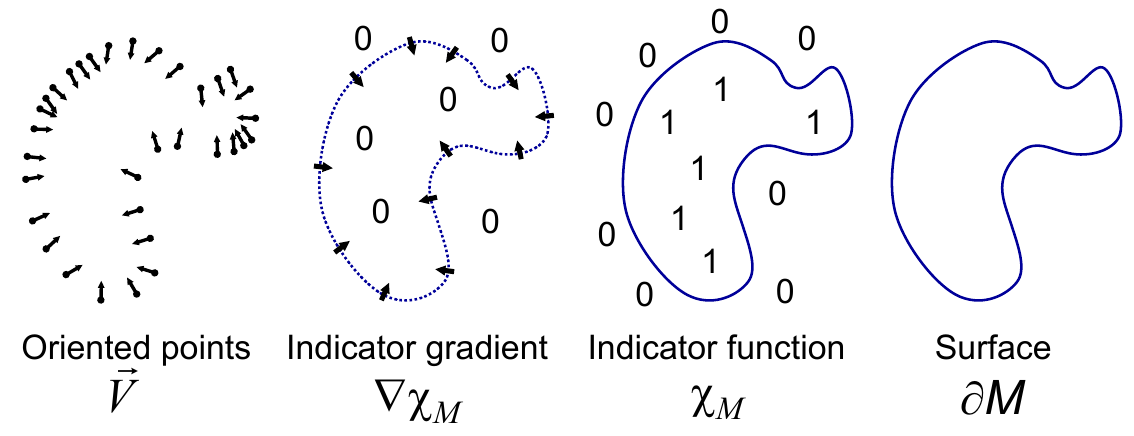
\includegraphics[width=0.7\textwidth]{poisson.png}
\caption{Intuitive illustration of Poisson reconstruction in 2D~\cite{poisson}.}
\label{fig:poisson}
\end{figure}

In detail, as illustrated in figure~\ref{fig:poisson} the already computed surface normals correspond to a vector field $\vec V$, which equals the gradient of the indicator function $\chi_M$. This is true, since the indicator function is constant everywhere except at the object's surface.

The points with the corresponding normals can thus be viewed as samples of the gradient of the indicator function. This results in the problem of finding the scalar function $\chi_M$, whose gradient best approximates the vector field $\vec V$ of the point cloud, i.e. $min_\chi \Arrowvert \nabla \chi_M-\vec V\Arrowvert$. Applying the divergence operator leads to desired poisson equation:
%
\begin{equation}
\Delta\chi\;=\;\nabla\vec V\,.
\end{equation}
%
Under creation of an octree data structure the mesh can finally be extracted, by detecting which egdes of the voxel are intersected by the model’s isosurface~\cite{possion2}.

\item \textbf{Organized fast mesh}\\
The organized fast mesh algorithm does essentially the same as the explained plane geometry algorithm in section~\ref{sec:planegeometry} and is therefore not described in more detail at this point.
%
\end{itemize}
%
\subsubsection*{\color{darkred}Implementation and usage}
%
For a detailed description of the parameters of the different methods the reader is encouraged to have a look at the documentation of PCL~\cite{pcldoc}. Most of the parameters are set by default to appropriate values (see \textit{processing.hpp}).
%
\paragraph*{Filters}
%
\begin{itemize}
\item \textbf{\texttt{void medianFilter(pcl::PointCloud<pcl::PointXYZ>::Ptr \&pcptr,\\std::string method, int window\_size, float max\_allowed\_movement)}}\\
\textsf{Median filter applied on the intensity depth map of the cloud.}
\item \textbf{\texttt{void bilateralFilter(pcl::PointCloud<pcl::PointXYZ>::Ptr \&pcptr,\\std::string method, double sigmaS, double sigmaR)}}\\
\textsf{Bilateral filter applied on the intensity depth map of the cloud.}
\end{itemize}
%
\paragraph*{Normal estimation}
%
\begin{itemize}
\item \textbf{\texttt{pcl::PointCloud<pcl::Normal>::Ptr leastsquareNormalEstimation\\(pcl::PointCloud<pcl::PointXYZ>::ConstPtr pcptr, std::string method,\\int k, double radius, bool openmp)}}\\
\textsf{Normal estimation via least-square plane fitting, whereby the variable openmp can be set to perform with OpenMP.}
\item \textbf{\texttt{pcl::PointCloud<pcl::Normal>::Ptr integralimagesNormalEstimation\\(pcl::PointCloud<pcl::PointXYZ>::ConstPtr pcptr, std::string method,\\int art, float max\_depth\_change\_factor, float normal\_smoothing\_size,\\bool depth\_dependent\_smoothing)}}\\
\textsf{Normal estimation via integral images, whereby the variable art defines the particular method: COVARIANCE\_MATRIX[0], AVERAGE\_3D\_GRADIENT [1], AVERAGE\_DEPTH\_CHANGE [2], SIMPLE\_3D\_GRADIENT [3]. The last method works like the previous, without averaging, thus no integral image is computed.}
\end{itemize}
%
\paragraph*{Mesh reconstruction}
%
\begin{itemize}
\item \textbf{\texttt{pcl::PolygonMesh gptGenerateMesh(pcl::PointCloud<pcl::PointNormal>\\::ConstPtr pcnormptr, std::string method, double mu, double radius,\\int nnn, double minimum\_angle, double maximum\_angle, double\\eps\_angle, bool consistent, bool consistent\_ordering)}}\\
\textsf{Greedy projection triangulation}
\item \textbf{\texttt{pcl::PolygonMesh poissonGenerateMesh(pcl::PointCloud<pcl::Point\\Normal>::ConstPtr pcnormptr, std::string method, int depth, int\\min\_depth, float point\_weight, float scale, int solver\_divide,\\int iso\_divide, float samples\_per\_node, bool confidence, bool\\output\_polygons, int degree, bool manifold)}}\\
\textsf{Poisson mesh reconstruction}
\end{itemize}
%
\subsection{Tools}
%
\subsubsection*{\color{darkgreen}Theorectial issues}
%
For a better understanding of the data and the processing methods the file \textit{tools.cpp}, included by \textit{tools.hpp}, contains some particular functions for getting information about the point cloud, which are useful for setting typical parameters and for cropping the cloud. Since some processing procedures need a lot of computation time for big point clouds, the cropping tool is convenient for the variation of input parameters while keeping the point density constant.
%
\subsubsection*{\color{darkred}Implementation and usage}
%
\begin{itemize}
\item \textbf{\texttt{int countEntries(pcl::PointCloud<pcl::PointXYZ>::ConstPtr pcptr)}}\\
\textsf{Returns the number of points, which are defined, i.e. $z\neq0$.}
\item \textbf{\texttt{void getSize(pcl::PointCloud<pcl::PointXYZ>::ConstPtr pcptr)}}\\
\textsf{Prints the spatial extension of the point cloud.}
\item \textbf{\texttt{void crop(pcl::PointCloud<pcl::PointXYZ>::Ptr \&pcptr, float x, float y, float dx, float dy)}}\\
\textsf{Crops a cube out of a point cloud with the center $x$, $y$, $z$ and the spatial extension $dx$, $dy$, $dz$.}
\item \textbf{\texttt{void crop(pcl::PointCloud<pcl::PointXYZRGB>::Ptr \&pcrgbptr, float x,\\float y, float dx, float dy)}}\\
\textsf{Crops a cube out of a colored point cloud with the center $x$, $y$, $z$ and the spatial extension $dx$, $dy$, $dz$.}
\item \textbf{\texttt{void cropAndShow(pcl::PointCloud<pcl::PointXYZ>::Ptr \&pcptr,\\pcl::PointCloud<pcl::PointXYZRGB>::Ptr \&pcrgbptr)}}\\
\textsf{One can choose via the spatial coordinates a region of the cloud and view this region to decide, whether the corresponding part should be cropped or not.}
\item \textbf{\texttt{double equals(pcl::PointCloud<pcl::PointXYZ>::Ptr \&pcptr1,\\pcl::PointCloud<pcl::PointXYZ>::Ptr \&pcptr2)}}\\
\textsf{Returns the fraction of equal points of two input point clouds.}
\item \textbf{\texttt{void center(pcl::PointCloud<pcl::PointXYZ>::Ptr \&pcptr,\\Eigen::Vector3f \&centroid)}}\\
\textsf{Computes the center neglecting undefined points (points with $z\neq0$).}
\item \textbf{\texttt{double calcMeanMin(pcl::PointCloud<pcl::PointXYZ>::Ptr \&pcptr,int k)}}\\
\textsf{Returns the mean minimum distance and computes its standard deviation between the points and their k-nearest neighbours.}
\item \textbf{\texttt{void info(pcl::PointCloud<pcl::PointXYZ>::Ptr \&pcptr)}}\\
\textsf{Gives some information about the point cloud.}
\end{itemize}
%
\subsection{Saving and postprocessing}
\subsubsection*{\color{darkgreen}Theorectial issues}
%
For a convenient handling of the generated data, and especially being able to work with the data in other application, it has to be possible to save, load and postprocess the data to appropriate formats. The pyl-files are saved in the folder \textit{data/plyfiles} and the especially modulated files for Three.js are stored separately at \textit{data/threejsfiles}. The following methods are provided.
%
\subsubsection*{\color{darkred}Implementation and usage}
%
\begin{itemize}
\item \textbf{\texttt{void save(std::string filename, pcl::PointCloud<pcl::PointXYZ>::Con\\stPtr xyz, pcl::PointCloud<pcl::PointXYZRGB>::ConstPtr xyzrgb,\\pcl::PointCloud<pcl::PointNormal>::Ptr xyznormal, pcl::Polygon\\Mesh \&mesh)}}\\
\textsf{Saves the point cloud and other 3D objects to file in \textit{data/plyfiles}, where a \textit{main file} is generated, which is stored at \textit{data} and has the nomenclature \textit{filename.pcl} containing all generated ply-files of this particular cloud.}
\item \textbf{\texttt{void load(std::string filename, pcl::PointCloud<pcl::PointXYZ>::Ptr\\xyz, pcl::PointCloud<pcl::PointXYZRGB>::Ptr xyzrgb, pcl::PointCloud\\<pcl::PointNormal>::Ptr xyznormal, pcl::PolygonMesh \&mesh)}}\\\textsf{Loading a cloud from file with the filename and store data in the corresponding objects, if available.}
\item \textbf{\texttt{void buildthreejsdata(std::string filename)}}\\
\textsf{Builds with the help of the following for functions out of the pcd-files all necessary files for a usage of the 3D objects with Three.js (saved with the suffix \textit{.three}).}
\item \textbf{\texttt{void compute\_xyz(std::string filename, const int width, const int\\height) }}\\
\textsf{Builds a file maintaining the spatial components of the point cloud for Three.js.}
\item \textbf{\texttt{void compute\_rgb(std::string filename, const int width, const int\\height)}}\\
\textsf{Builds a file maintaining the color components of the point cloud for Three.js.}
\item \textbf{\texttt{void compute\_faces(std::string filename, const int width, const int\\height)}}\\
\textsf{Builds a file maintaining the faces of the polygon mesh for Three.js.}
\item \textbf{\texttt{void compute\_normals(std::string filename, const int width, const\\int height)}}\\
\textsf{Builds a file maintaining the normals of the point cloud for Three.js.}
\end{itemize}
%
\section{Three.js - Loading and visualizing point clouds}
%
Looking for a more comfortable way to visualize the generated 3D objects, Three.js~\cite{three} turned out to be a very useful tool. As a web application it can be used with every browser and no addition libraries or programs have to be installed. Being inspired by the already implemented \textit{Android Lens Blur Depth Viewer} presented at~\cite{depthplayer}, some code pieces and ideas could be adapted for the aim of an easy way of illustration.

With the preprocessing of pcl and c++ at \textit{data/threejsfiles} the ply-files containing spatial and color information as well as normals and faces of a reconstructed mesh can be found with the ending \textit{.three}. For an easy handling with Three.js the data is stored separately. That means, that each file contains only the information it is named to. Acutally each ply-file is saved as a xyz-cloud and the data is reallocated with javascript to their correct content. This kind of structuring also prevents loading redundant data.

Loading data is not so easy in javascript, since it is difficult to access the full file path (probably for security reasons) and to load text files. Accordingly it was chosen a fixed file structure and the \textit{main files} for loading a point cloud are saved under \textit{data}, again with the ending \textit{.three}, where the name of the file already contains all necessary information for loading the correct files in javascript. These are the name, the width and height of the ordered point cloud and the following four letters indicate whether a the spatial coordinates ($x$), color information ($c$), normals ($n$) and faces ($f$) are loadable. Putting another letter on such a position (for example an $o$) means, that this information is not given. 

The main web application \textit{depthdataviewer.html} can be opended with a browser. The necessary js-files for usage of the Three.js library, loading the 3D objects, and blurring the depth image are stored in the \textit{lib} folder.
%
\subsection{General usage}
%
With the fixed structure the files for loading the point clouds under Three.js can be found in \textit{data} with the ending \textit{.three}. Corresponding to the present information (spatial, color, normals, faces) the cloud can be loaded via the \textit{Durchsuchen...} button. Having loaded the data below \textit{2D Illustrations} the depth image can be seen on the left and the color image on the right side in the panel. The \textit{Reload Page} button does what it is named after.

For different presentations of the point cloud one can choose below \textit{Render Mode} between visualization of the point cloud and the mesh. Furthermore the point size can be changed, normals can be viewed and it is possible to see only the wireframe of the mesh. If a mesh without normals was loaded, the vertex normals are computed via Three.js out of the faces. In the following text window information about the current processes is given.

The last two subitems, \textit{Plane Geometry} and \textit{StackBlur Method}, are further methods for processing the point cloud and are explained in the next two subsections, whereby the \textit{plane geometry} can be loaded via the corresponding button and the blurring with a given smoothing radius can be enabled/disabled.
%
\subsection{Plane geometry}
\label{sec:planegeometry}
Like already mentioned plane geometry is a special method for processing. Especially one generates a mesh out of an ordered point cloud. The idea is to place a lattice upon the depth image with a side length of adjacent points, where each square is divided into two triangles (faces). According to their depth data the lattice points are placed perpendicular to the depth image plane. Loading the plane geometry even though a mesh was already loaded, the present mesh is deleted and replaced by the plane geometry. The same holds if no normals were loaded.
%
\subsection{Stack blur}
%
The stack blur algorithm is adopted from~\cite{stack} and can be used to blur the depth image to gain smoother surfaces. Similar to the bilateral filter the algortihm is based on a Gaussian Blur implementation. It presents a nice visible \textit{toy tool} for processing.
%
\section{Discussion}
%
For a simple handling of 3D data some useful methods for preparaing a depth dataset, visualization and processing of the data as well as the reconstruction of a mesh out of a point cloud were implemented with PCL and Three.js. Within the project a detailed investigation of the parameters of the processing steps and therefore an evaluation of the different methods was not possible due to the addition effort of time, but definitly should be done. In addition to the already mentioned extensions, briefly a view problems of the project, which are not solved yet, as well as some suggestions for improvement are stated:
%
\begin{itemize}
 \item Currently the clouds are mainly passed to the function via call by reference with pointers. This is not usual anymore and one should consider to use smart pointers instead.
 \item The renderer of Three.js seems to have problems to visualize some objects. In particular the objects are loaded, but not visible in the application. Either the renderer just has to be refreshed at the end of the loading process or the reasons are more complicated. Therefore and due to the lack of knowledge in javascript programming this problem has not been fixed, yet.
 \item A similar problem arises when illustrating the wireframe of the plane geometry. For some reason often only one side of the wireframe is displayed.
 \item The information panel of the web application should give some more information about the current processes/changes. In addition it could be possible to extend it to a terminal for directly typing commands. However, a direct connection to the PCL applications is probably not possible.
\end{itemize}
%
In its expandability and applicability the implementations of the project certainly have a vast spectrum of possible improvements for a more general and abstract handling. However, as a first attempt, it turnes out to contain the main necessary functions and it could be used for a faster access to the structure and usage of PCL and three.js.
\newpage
\begin{thebibliography}{185}

\bibitem{bilateral}C. Tomasi, R. Manduchi, \textit{Bilateral Filtering for Gray and Color Images}, Proceedings of the Sixth International Conference on Computer Vision, 1998, 839

\bibitem{poisson}Michael Kazhdan1, Matthew Bolitho1 and Hugues Hoppe2, (2006), \textit{Poisson surface reconstruction}, Symposium on Geometry Processing, 2006, 61-70

\bibitem{greedy}Matthew T. Dickersony, Robert L. Scot Drysdalez, Scott A. McElfresh and Emo Welzl, \textit{Fast Greedy Triangulation Algorithms}, 1994

\bibitem{integral}S. Holzer, R. B. Rusu, M. Dixon, S. Gedikli and N. Navab1, \textit{Adaptive Neighborhood Selection for Real-Time Surface Normal, Estimation from Organized Point Cloud Data Using Integral Images}, IEEE/RSJ International Conference on Intelligent Robots and Systems, 2012

\bibitem{tuzel}F. Porikli and O. Tuzel, \textit{Fast Construction of Covariance Matrices for Arbitrary Size Image Windows}, IEEE International Conference on
Image Processing, 2006


{\textbf{Bachelor Thesis}}

\bibitem{recon}Juha Hyvärinen, (2012), \textit{Surface reconstruction of point clouds captured with microsoft kinect}, Oulu University of Applied Sciences, Degree Programme in Information Technology and Telecommunications

{\textbf{Internet sources}}

\bibitem{pcldoc}PCL Documentation, URL: \url{http://pointclouds.org/documentation/} (Visited March 2016)

\bibitem{peris}Martin Peris Blog, URL: \url{http://blog.martinperis.com/2012/01/3d-reconstruction-with-opencv-and-point.html} (Visited March 2016)

\bibitem{depthplayer}Click To Release Blog from Jaume Sanchez, URL: \url{https://www.clicktorelease.com/code/depth-player/} (Visited March 2016)

\bibitem{ordered}Software Support Center, URL: \url{http://support1.geomagic.com/link/portal/5605/5668/Article/1130/Should-I-work-with-ordered-or-unordered-points} (Visited March 2016)

\bibitem{possion2}3D Scan 2.0, TU Freiburg, URL: \url{http://vr.tu-freiberg.de/scivi/?page_id=365} (Visited March 2016)

\bibitem{three}Javascript 3D Library, URL: \url{http://threejs.org/} (Visited March 2016)

\bibitem{stack}Quasimondo, URL: \url{http://www.quasimondo.com/StackBlurForCanvas/StackBlurDemo.html} (Visited March 2016)

\end{thebibliography}
\end{document}